\documentclass{beamer}

% latex commands and macros

% common sets
\newcommand{\R}{\mathbb{R}} % the set of real numbers
\newcommand{\C}{\mathbb{C}} % the set of complex numbers
\newcommand{\Z}{\mathbb{Z}} % the set of integers
\newcommand{\N}{\mathbb{N}} % the set of natural numbers
\newcommand{\Q}{\mathbb{Q}} % the set of rational numbers
\newcommand{\F}{\mathbb{F}} % usually stands for field
\newcommand{\D}{\mathbb{D}} % the unit disc in the complex plane
\newcommand{\B}{\mathbb{B}} % the unit ball
\newcommand{\es}{\mathbb{S}} % sphere
\newcommand{\T}{\mathbb{T}} % torus
\newcommand{\RP}{\mathbb{R}P} % projective plane
\newcommand{\CP}{\mathbb{C}P} % complex projective plane
\DeclareMathOperator \Gr {Gr} % grassmannian
\newcommand{\ham}{\mathbb{H}} % quaternions

% common operations and connectors
\newcommand{\inner}[2]{\left<{#1},\,{#2}\right>} % inner product
\newcommand{\coset}[1]{\left<{#1}\right>} % groups or ideal generated by some set
\newcommand{\norm}[1]{\left\|{#1}\right\|} % norm of a vector
\newcommand{\abs}[1]{\left|{#1}\right|} % absolute value
\newcommand{\sets}[1]{\left\{{#1}\right\}} % a simple set with no conditions
\newcommand{\set}[2]{\sets{{#1}:\,{#2}}} % a set with conditions
\newcommand{\prn}[1]{\left({#1}\right)} % parentheses 
\newcommand{\brak}[2]{\left[{#1},\,{#2}\right]} % bracket product
\newcommand{\pbrak}[2]{\left\{{#1},{#2}\right\}} % Poisson bracket product

\DeclareMathOperator \csum {\#} % connected sum

\DeclareMathOperator \pp {\,a.e.} % almost everywhere
\DeclareMathOperator \sgn {sgn} % signum function
\DeclareMathOperator \spn {span} % span
\DeclareMathOperator \cspn {\overline{span}} % closed span
\DeclareMathOperator \img {Im} % imaginary part of a complex number
\DeclareMathOperator \rea {Re} % real part of a complex number
\DeclareMathOperator \ind {ind} % index of a function
\DeclareMathOperator \diam {diam} % diameter of a set or a graph
\DeclareMathOperator \res {res} % residue of a complex function
\DeclareMathOperator \dist {dist} % distance function
\DeclareMathOperator \wind {wind} % winding number
\DeclareMathOperator \spectrum {\sigma} % spectrum of an operator
\DeclareMathOperator \spectrumEssential {\sigma_{\text{ess}}} % essential spectrum of an operator

\DeclareMathOperator \smb {smb} % symbol $C^*$-homomorphism

\newcommand{\acton}[2]{\phantom{|}^{{#1}}{{#2}}} % hack to prepend a superscript

\DeclareMathOperator \Syl {Syl} % Sylow subgroup
\DeclareMathOperator \im {im} % image of a function
\DeclareMathOperator \Tor {Tor} % torsion
\DeclareMathOperator \Aut {Aut} % automorphisms
\DeclareMathOperator \End {End} % endomorphisms
\DeclareMathOperator \Mod {Mod} % modules
\DeclareMathOperator \Hol {Hol} % holomorphic functions
\DeclareMathOperator \Sym {Sym} % symmetric group
\DeclareMathOperator \Alt {Alt} % alternating groups
\DeclareMathOperator \Mat {Mat} % matrices
\DeclareMathOperator \Spec {Spec} % spectrum of a ring
\DeclareMathOperator \Max {Max} % maximal spectrum of a ring
\DeclareMathOperator \coker {coker} % cokernel
\DeclareMathOperator \GL {GL} % general linear group
\DeclareMathOperator \SL {SL} % special linear group
\DeclareMathOperator \codim {codim} % codimension of a vector subspace
\DeclareMathOperator \rnk {rnk} % rank of a linear transform
\DeclareMathOperator \Id {Id} % identity function
\DeclareMathOperator \Tr {Tr} % trace of a matrix
\DeclareMathOperator \diag {diag} % diagonal matrix
\DeclareMathOperator \supp {supp} % support of a function

% category theory
\DeclareMathOperator \Ob {Ob} % objects
\DeclareMathOperator \Mor {Mor} % morphism
\DeclareMathOperator \Hom {Hom} % homomorphisms
\DeclareMathOperator \Lin {\mathbf{Lin}} % linear
\DeclareMathOperator \Set {\mathbf{Set}} % sets
\DeclareMathOperator \Vect {\mathbf{Vect}} % vector spaces

% vector calculus
\DeclareMathOperator \diver {div} % divergence
\DeclareMathOperator \grad {grad} % gradient
\DeclareMathOperator \curl {curl} % curl

\DeclareMathOperator \Lie {Lie} % Lie groups
\newcommand{\lie}[1]{\mathfrak{{#1}}} % lie algebra

% operator analysis
\newcommand \slim {\text{s-}\lim} % strong limit
\DeclareMathOperator \Fl{\mathbb{F}l} % spaces of frequency weighted norms
\DeclareMathOperator \Smb{Smb} % symbol operator
\DeclareMathOperator \Alg{Alg} % algebra generated by a set

% statistics
\DeclareMathOperator \Exp{\mathbb{E}} % variance
\DeclareMathOperator \Var{Var} % variance

% miscellaneous

% frequently used abbreviations
\newcommand{\ve}{\varepsilon} % epsilon clearly distinguishable from inclusion
\newcommand{\vf}{\varphi} % more popular way of writing phi
\newcommand{\vn}{\varnothing} % the empty set

% special notation for dissertation
\newcommand{\hprod}{\circ} % Hadamard or entrywise multiplication of matrices
\newcommand{\hs}{{\mathcal{C}_2}} % Hilbert-Schmidt class
\newcommand{\poi}{{\mathcal{P}_1}} % Poincare class
\newcommand{\MellinTransform}{\mathcal{M}} % Mellin Transform
\newcommand{\MellinConvolution}{*_{\MellinTransform}} % Mellin convolution

% environments and fonts for cifar-ten project
\newcommand{\code}[1]{\texttt{{#1}}}

% styles of theorems, definitions and remarks
\theoremstyle{plain}
\newtheorem{thm}{Theorem}%[section]
\newtheorem{lemma}[thm]{Lemma}
\newtheorem{prop}[thm]{Proposition}
\newtheorem{cor}[thm]{Corollary}
\newtheorem{axiom}[thm]{Axiom}
\newtheorem{exercise}[thm]{Exercise}
\newtheorem{claim}[thm]{Claim}
\newtheorem{fact}[thm]{Fact}

\theoremstyle{definition}
\newtheorem{defn}[thm]{Definition}

\theoremstyle{remark}
\newtheorem{remark}[thm]{Remark}
\newtheorem{exmpl}[thm]{Example}
\newtheorem{problem}[thm]{Problem}
\newtheorem{prob}[thm]{Problem}
\newtheorem{fle}[thm]{File}

% page format
\oddsidemargin=0in
\evensidemargin=0in
\textwidth=6in
\topmargin=-0.5in
\textheight=9.5in
\parindent=.375in

% packages
\usepackage{enumerate}
\usepackage{amssymb}
%\usepackage[all,cmtip]{xy}
\usepackage[mathscr]{eucal}
\usepackage{graphicx,color}

\newcommand{\titleChaos}[1]{\title[HW {#1}]{Introduction to Chaos, Homework {#1}}}

%\begin{figure}[ht]
%       \includegraphics[height=1in,keepaspectratio]{03NegativeHelix.jpg}
%       \caption{Negative writhe crossings} \label{fig:negativeWritheCrossings}
%\end{figure}


% packages
\usepackage{beamerthemesplit}
\usepackage{enumerate}
\usepackage{amssymb}
\usepackage[all,cmtip]{xy}
\usepackage[mathscr]{eucal}
\usepackage[natbib=true,style=authoryear,backend=bibtex,useprefix=true]{biblatex}
\addbibresource{reading.bib}
\usepackage{graphicx,color}

\title{AlphaFold Bitesized Pieces}
\author{Reuben Brasher}
\date{\today}

\begin{document}

\frame{\titlepage}

\section[Outline]{}
\frame{\tableofcontents}

\section{ML Nutshell}
\frame
{
   \frametitle{How to be an ML Engineer}

   \begin{itemize}
      \item<1-> Define cost function

      \item<2-> Define network architecture
      
      \item<3-> Apply gradient descent
      
   \end{itemize}
}

\frame
{
   \frametitle{Classical Neural net}
   
   Refer to Fig. \ref{fig:neuralnet}.
   
   \begin{figure}[ht]
      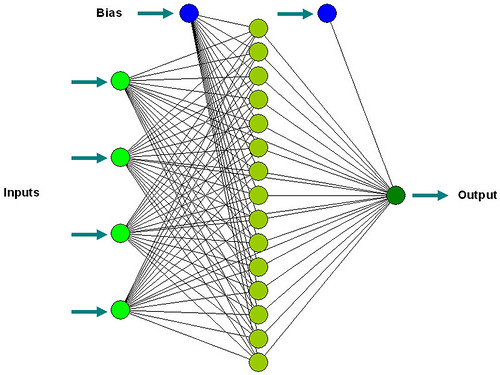
\includegraphics[height=2in,keepaspectratio]{images/7880863848_0698ba4909.jpg}
      \caption{https://search.creativecommons.org/photos/70ab8654-c234-4dbe-9b1c-62851544245a} \label{fig:neuralnet}
   \end{figure}
}

\frame
{
   \frametitle{Dense Layers}

   \begin{itemize}
      \item<1-> Linear function whose coefficients are parameters of model

         $$y_j = \sum_i w_{ij} x_{ij} + b_j$$

      \item<2-> Possible non-linear activation function

         $$F(y)$$

         or

         $$f(y_j)$$

   \end{itemize}
}

\frame
{
   \frametitle{Common activation functions, tanh and sigmoid}

   $$\tanh(x) = \frac{e^x - e^{-x}}{e^x + e^{-x}}$$
   $$\sigmoid(x) = \frac{1}{1 + e^{-x}}$$
}


\frame
{
   \frametitle{Common activation functions, softmax}

   $$\softmax(x)_j = \frac{e^{x_j}}{\sum_i e^{x_i}}$$
}

\frame
{
   \frametitle{Common activation functions, relu}

   $$\relu(x) = \max(x, 0)$$
}

\frame
{
   \frametitle{Gate Layers}

   \begin{itemize}
      \item<1-> Entrywise multiplication of two previous layers outputs

      $$(x \odot y)_i = x_i y_i$$

      \item<2-> Became popular with LSTM and GRU
      
   \end{itemize}
}

\frame
{
   \frametitle{Attention Layers}

   \begin{itemize}
      \item<1-> Define a convex combination along axis of previous layer

      $$y_i = F(x_i)$$

      $$a_i = \softmax(\linear(y))_i$$

      $$\sum_i a_i y_i$$

      \item<2-> Became popular with question answering methods.
      
   \end{itemize}
}

\frame
{
   \frametitle{Transformers with Multi-head Attention Layers}

   \begin{itemize}
      \item<1-> Multi-head attention. Layer produces three outputs $q$, $k$ and $v$

      $$\softmax ({qk^T}) v$$

      \item<2-> Defined in \cite{vaswani2017attention}
      
   \end{itemize}
}

\frame
{
   \frametitle{Gradient descent}

   $\phi$ a real-valued function of net output $F(x)$ and possible labeled observation $y$

   $\Theta$ the parameters (linear coefficients)

   Cost is
   $$\phi(F(x|\Theta), y)$$

   Minimize with respect to parameters using gradient 

   $$\nabla_\Theta \phi(F(x|\Theta), y)$$
}

\frame
{
   \frametitle{Encoder-decoder pattern}

   Train a pair of models, encoder to produce concise representation and decoder to reconstruct.

   Later encoder and decoder can be used separately. 
}

\section{Inspiration Papers}

\frame
{
   \frametitle{Bert: Pre-training of deep bidirectional transformers for language understanding}

   \cite{devlin2018bert}

   Model pretrained to reconstruct corrupted text and then finetuned
}

\frame
{
   \frametitle{Human pose estimation with iterative error feedback}

   \cite{carreira2016human}

   
}

\frame
{
   \frametitle{Self-training with noisy student improves imagenet classification}

   \cite{xie2020self}

   % equations
}

\frame
{
   \frametitle{Deep residual learning for image recognition}

   \cite{he2016deep}

   % equations
}

\begin{frame}[t,allowframebreaks]
\frametitle{References}
\printbibliography
\end{frame}

\end{document}
